\documentclass{article}

\usepackage{amsmath, amssymb, graphicx}
\usepackage{tikz}
\usepackage{listings}
\lstset{basicstyle=\ttfamily}
\title{Regular Path Queries in Graph Databases}
\date{\today}
\author{Lewis Dyer}

\begin{document}
\maketitle

Regular path queries are a common formalism to describe paths in graph databases under certain constraints. In particular, regular path queries describe constraints on paths by forming words from paths based on the edge labels included in these paths, and accept paths whose words are accepted by some regular expression $r$. The remainder of this paper is structured as follows. In Section \ref{sec:prelims}, we introduce some preliminary notions from graph and automata theory, while in Section \ref{sec:intro_rpqs} we formally introduce regular path queries, discuss where regular path queries are used in practice, and consider various different semantics for evaluating regular path queries. In Section \ref{sec:complexity} we consider the complexity of several variants of the evaluation problem on regular path queries, and in Section \ref{sec:simple_characterisation} we discuss various methods for characterising regular path queries when looking for simple paths between two vertices. Finally, in Section \ref{sec:future_work} we briefly discuss some potential future directions for research in regular path queries.

\begin{itemize}
    \item Formally define Regular Path Queries, and give an example or two.
    \item Formally introduce the main semantics of regular path queries, defining the main algorithmic questions in play.
    \item Give some results so far.
\end{itemize}

\section{Preliminaries}
\label{sec:prelims}

As a model for graph databases, we consider directed edge-labelled graphs. Given an alphabet $\Sigma$, a graph $G = (V,E)$ consists of a set of vertices $V$, along with a set of edges $E \subseteq (V \times \Sigma \times V)$, with $(u, l, v)$ denoting at edge from vertex $u$ to vertex $b$ with label $l$. Note that this model requires that every edge is labeled, and that we may omit the label if this label is irrelevant or clear from context. We further note that loops and multiple edges are permitted in this model.

Given two vertices $u$ and $v$, a path $p$ is defined by a sequence of edges of the form $(v_0, l_1, v_1), (v_1, l_2, v_2), \dots, (v_{n-1}, l_n, v_n)$ where $u = v_0$ and $v = v_1$, and we say this path has length $n$. We denote $\mathcal{P}_(G, u ,v)$ as the set of all such paths in $G$ between $u$ and $v$, occasionally omitting the subscript where this is clear from context.  We say a path is $\emph{simple}$ if any two vertices $v_i, v_j$ in $p$ are pairwise distinct.

Given an alphabet $\Sigma$, we define a regular expression $r$ as follows. First, the empty string $\epsilon$ is a regular expression, along with any character $a$ with $a \in \Sigma$. Then, given two regular expressions $r$ and $s$, their concatenation $(rs)$, denoting the set of strings obtained by concatenating a string accepted in $r$ and a string accepted by $s$, is also a regular expression. Their alternation $(r | s)$, denoting the set of strings accepted by $r$ or $s$, is also a regular expression, along with $(r^*)$, the set of finite strings obtained by concatenating zero or more strings which are recognised by $r$. We also allow for ommitting parentheses where there is no ambiguity. We say the \emph{language} of $r$, denoted $L(r) \subset \Sigma^*$, is the set of strings which are accepted by $r$.

Regular expressions can also be described using nondeterministic finite automata (or an NFA for short), which are tuples of the form $N = (Q, \Sigma, \Delta, Q_0, Q_1)$. Here $Q$ is a finite set of states in the automata, $\Sigma$ is a finite alphabet as for regular expressions, $Q_0$ is a set of initial states in $Q$, $Q_1$ is a set of accepting states in $Q$, and $\Delta \subseteq Q \times \Sigma \times Q$ representing transitions between states, such that $(q, a, q')$ represents a transition from $q$ to $q'$ via the character $a$. Note that nondeterminism here means that a single state may have multiple transitions to different states using the same character. We may also define the product of a graph $G$ with start and end vertices $s$ and $t$ and a nondeterministic finite automata $N$, which is a graph $G \times N$ such that $V(G \times N) = V \times Q$ and $E(G \times N) = \{((u_1, q_1), a, (u_2,q_2)) | (u_1, a, u_2) \in E \text{ and } (q_1, a, q_2) \in Delta$. In other words, an edge with label $a$ exists between two vertex-state pairs if and only if an edge with label $a$ exists between both vertices in $G$, and moreover there exists a transition in $N$ between both states with label $a$. We further note that this may also be treated as an NFA by treating the sets of vertices and edges as the set of states and transitions respectively, and by defining $Q_0 = \{(s, q) | q \in Q\}$ and $Q_1 = \{(t, q) | q \in Q\}$.

\section{Introducing regular path queries}
\label{sec:intro_rpqs}

Given a path $p$ in a graph $G$ and vertices $u$ and $v$, we consider the word $w_p$ formed in $\Sigma^*$ by concatenating each edge label in $p$. More formally, the function $w: \mathcal{P}_{(G,u,v)} \rightarrow \Sigma^*$ with $w \left((v_0, l_1, v_1), (v_1, l_2, v_2), \dots, (v_{n-1}, l_n, v_n) \right) = l_1 l_2 \dots l_n$ produces the unique word associated with a given path $p$. Regular path queries (also denoted as RPQs) consist of a regular expression $r$ along with a set of \emph{semantics} for that RPQ, though we frequently refer to an RPQ solely by the regular expression where the semantics being used are clear from context. Evaluating an RPQ over a graph $G$ between vertices $u$ and $v$ consists of two steps: first, we consider paths $p \in \mathcal{P}_{(G,u,v)}$ such that $w(p)$ is accepted by $r$, and we denote these paths as the set of \emph{candidate paths} of the RPQ. Then, we determine which of these candidate paths to output depending on the semantics being used. Three typical sets of semantics are:

\begin{itemize}
    \item \textbf{Arbitrary semantics}, where all candidate paths are returned.
    \item \textbf{Shortest path semantics}, where all candidate paths of minimum length are returned.
    \item \textbf{Simple path semantics}, where all simple candidate paths are returned.
\end{itemize}

\begin{figure}
    \centering
    \label{fig:arbitrary_infinite}
    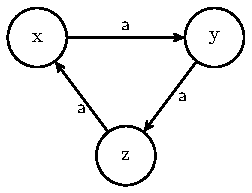
\includegraphics{figures/arbitrary_infinite.pdf}
    \caption{A directed cyclic graph on $3$ vertices, where every edge has label $a$.}
\end{figure}

Each of these sets of semantics presents different challenges. When using arbitrary semantics, care must be taken to avoid paths of infinite length, which can occur in cyclic directed graphs. For example, evaluating $a^*$ over the graph in Figure \ref{fig:arbitrary_infinite} from vertex $x$ to vertex $y$ using arbitrary semantics will result in an infinite set of paths with words given by the set $\{a^{3k+1} | k \in \mathbb{N}\}$.

Shortest path semantics avoid this problem, but can be counter-intuitive even for common queries. For example, when counting the number of paths between two vertices $x$ and $y$ that are accepted by some regular expression $r$, adding an additional path between $x$ and $y$ can actually reduce the overall count, if this newly added path is accepted by $r$ and is shorter than any other paths.

Simple paths avoid this lack of intuition while also avoiding paths of infinite length, and correspond to many natural constraints on paths in common queries. For example, in a transport network where vertices correspond to locations and edges correspond to different forms of travel between locations, finding simple paths between two locations means that visiting the same location more than once is not permitted.

Regular path queries are applied in SPARQL, a database query language providing specific syntax for graph traversals, via the use of \emph{property paths} \cite{SPARQLQueryLanguage}. For example, the following query from the Wikidata knowledge graph \cite{WikidataSPARQLQuery} uses such a property path:


\begin{lstlisting}[language=SPARQL]
SELECT ?siteLabel ?coord ?image ?site
WHERE {
   ?site wdt:P31/wdt:P279* wd:Q839954 ;
      wdt:P625 ?coord ;
      wdt:P18 ?image .
SERVICE wikibase:label { bd:serviceParam
wikibase:language "[AUTO_LANGUAGE],en".}
}
\end{lstlisting}

This query returns a list of all archaeological sites in the knowledge graph, along with their names, locations and an associated image. Most notably, \texttt{?site wdt:P31/wdt:P279* wd:Q839954} represents a regular path query between the vertex \texttt{?site}, representing a candidate instance of an archaeological site, and the vertex \texttt{wd:Q839954} representing the concept of an archaeological site, where any desired path consists of a sequence of edges with edge labels either \texttt{wdt:P31}, representing that an entity is an instance of a concept, or \texttt{wdt:P279} representing that one concept is a subclass of another concept. The need for a property path here arises because specific archaeological sites may not be adjacent to vertex \texttt{wd:Q839954}, and may be instances of more specific concepts instead. For example, Duncarnock Hill Fort is an instance of a contour fort, which is a subclass of hillforts which are in turn a subclass of ancient monuments, which are finally subclasses of archaeological sites. Hence, regular path queries are especially suited to knowledge graphs, or any sort of graph database with hierachical relationships between entities.

\section{Complexity of evaluating RPQs}
\label{sec:complexity}

To begin, we first formalise the set of evaluation problems on RPQs we are considering. We define the decision RPQ evaluation problem with arbitrary path semantics as follows:

\fbox{\parbox{\textwidth}{
\textsc{Path}

\textbf{Input:} A graph $G$ with a starting vertex $s$ and an ending vertex $e$, and a regular expression $r$.\\

\textbf{Output:} \texttt{true} if there exists a path $p$ in $G$ matching $s$ and $r$ such that $w(p)$ is accepted by $r$, and \texttt{false} otherwise.
}} \\

Note that this defines the decision problem for RPQ evaluation under arbitrary path semantics. Analogous variants of this decision problem exist for the other forms of semantics introduced in Section \ref{sec:intro_rpqs}, which we shall denote as \textsc{ShortPath} and \text{SimPath} for shortest path and simple path semantics respectively. Similarly, we may also define enumeration variants of these problems, where all such paths from $s$ to $r$ whose words are accepted by $r$ should be returned. We denote these problems as \textsc{EnumPaths}, \textsc{EnumShortPaths} and \textsc{EnumSimPaths}.

Firstly, we know that \textsc{Path} is solvable in polynomial time for any regular expression $r$. This follows by taking the product of $G$ and the NFA $N$ representing the regular expression $r$, and determining if there exists a path from $(s, q_0)$ to $(t, q_1)$, for some $q_0 \in Q_0$ and $q_1 \in Q_1$.

Considering this product as an NFA allows us to extend this procedure to solve \textsc{EnumPaths} in polynomial delay. Specifically, we produce a new NFA $N'$ by replacing all transitions of the form $((u_1, q_1), a, (u_2, q_2))$ with $((u_1, q_1), (u_1, a, u_2), (u_2, q_2))$, such that the set of labels $\Sigma$ now represents the set of transitions in $N$. Hence, enumerating paths from $s$ to $t$ such that their words are accepted by $r$ is equivalent to enumerating every word that is accepted by $N'$, which Ackerman and Shallit show in \cite{ackermanEfficientEnumerationWords2009} can be computed in polynomial delay. We further have that \textsc{EnumShortPaths} can also be computed in polynomial delay - since the algorithm introduced by Ackerman and Shallit returns words in radix order, we may simply just terminate when the length of a word accepted by $r$ is enumerated that is longer than the previous enumerated word.


\section{Characterising RPQs for simple path semantics}
\label{sec:simple_characterisation}

As discussed in Section \ref{sec:complexity}, \textsc{SimPath} and \textsc{EnumSimPaths} are in general intractable over all possible regular expressions, with \textsc{SimPath} being NP-complete with the regular expression $(aa)^*$ as shown by Lapaugh and Papadimitriou in \cite{lapaughEvenpathProblemGraphs1984}, and \textsc{EnumSimPaths} being \#P-complete with the regular expression $a^*$ as shown by Valiant in \cite{valiantComplexityComputingPermanent1979}. A natural further question is whether a particular class of regular expressions allows for tractable decision and enumeration, and moreover whether this class is sufficiently powerful to handle regular path queries that are used in practice.

Bagan et al. introduce a trichotomy for \textsc{SimPath} in \cite{baganTrichotomyRegularSimple2020}. Specifically, they define the family of tractable languages $C_{tract}$ as follows. A language is in $C_{tract}$ if and only if, for some $i \in \mathbb{N}$, we have that for any words $w_l, w_m, w_r$ and any non-empty words $w_1, w_2$, if $w_l w_1^i w_m w_2^i w_r \in L$ then it follows that $w_l w_1^i w_2^i w_r \in L$. For example, over the alphabet $\Sigma = \{a, b, c\}$, the regular language defined by the expression $ab^*$ is in $C_{tract}$, by taking $i=1$ and considering the cases where $w_l$ is empty or non-empty, arguing that $a$ must either be included in $w_1$ or $w_l$ respectively. The trichotomy then proceeds from this definition: \textsc{SimPath} is NP-complete for languages not in $C_{tract}$, NL-complete for infinite languages in $C_{tract}$, and in $AC^0$ for finite languages in $C_{tract}$.

Martens and Trauter tackle this question for \textsc{EnumSimPaths} in \cite{martensEvaluationEnumerationProblems2018} by defining the class of \emph{simple transitive expressions} (STEs for short). In this class, we define \emph{atomic expressions} as expressions of the form $(a_1 + \dots a_n)$ for $a_i \in \Sigma$, which we denote as $A$. Note that since the order of elements in this expression is unimportant, we also denote $A$ as a subset of $\Sigma$, such that $a_i \in A$ if and only if $a_i$ is accepted by $A$, and we also allow for $A$ to be the emptyset, in which case $\epsilon$ is the only string accepted by $A$. We then further define \emph{bounded expressions} as expressions of the form $A_1 \dots A_k$ or $A_1 ? \dots A_k ?$ for some $k \geq 0$ such that each $A_i$ is an atomic expression. Finally, a simple transitive expression is an expression of the form $B_{pre}A^* B_{post}$, such that $B_{pre}$ and $B_{post}$ are bounded expressions while $A$ is an atomic expression.

Intuitively, the main idea behind STEs is that a bounded amount of local navigation is permitted at the start and end of each expression, consisting of testing paths either of length exactly $k$ or with length at most $k$. Then, the optional transitive step in the middle of the expression is sufficiently simple.

Following this, Martens and Trauter define a dichotomy over classes of STEs using the notion of \emph{cuttability} - intuitively speaking, that parts of the expression which do not match the transitive part should only occur within a constant distance of the start or end of the expression. More precisely, we define the \emph{left cut border} of an STE $r$ as the largest value $c_l$ such that, for $B_{pre} = A_1 \dots A_k$, $T$ is not a subset of $A_{c_l}$, or zero if either this value does not exist or $B_pre$ is of the form $A_1 ? \dots A_k ?$. The right cut border $c_r$ is defined analogously, reversing the indices in $B_{post}$, and we say an expression has cut border $c$ if the maximum of its left and right cut borders is $c$, and in particular that a class of STEs $\mathcal{R}$ is \emph{cuttable} if there exists a constant $c$ such that every expression in $\mathcal{R}$ has cut border at most $c$. We also need one more mild condition on classes of STEs. Given some class of STEs $\mathcal{R}$, we say $\mathcal{R}$ can be sampled if there exists an algorithm that, given any $k$, either returns a expression in $\mathcal{R}$ whose cut border is greater than $k$, or else returns that such an expression does not exist.

Given this relatively mild condition, we obtain the following dichotomy: for any class of STEs $\mathcal{R}$ that can be sampled, if $\mathcal{R}$ is cuttable then $\textsc{SimPath}$ is $FPT$ over any $r \in \mathcal{R}$ parameterised by the length of $r$. Otherwise, $\textsc{SimPath}$ is W[1]-hard for any $r \in \mathcal{R}$.

While this dichotomy is powerful within the class of STEs, one notable shortcoming is that the class of STEs is quite a limited subset of regular expressions. For example, the regular expressions $a + b^+$ and $(ab)^*$ are not STEs. However, analysis of SPARQL query logs performed by Bonifati et al. in \cite{bonifatiAnalyticalStudyLarge2020} shows that $99.992\%$ of regular path queries in these query logs are STEs, and the vast majority of STEs in these query logs have cut border at most $2$, so in practice considering STEs covers both many common occurrences

Moving onto enumeration problems, Yen's algorithm \cite{yenFindingShortestLoopless1971} provides a polyomial delay algorithm to enumerate all simple paths between two vertices $s$ and $t$, without any sort of labelling on edges. Informally, this algorithm operates by finding a shortest path between $s$ and $t$, since any shortest path must also be a simple path. We then consider modifications of this path where the first $i$ edges coincide but the $(i+1)$th edge differs, continually repeating this procedure until all simple paths are found.

Returning to edge labelled graphs, Martens and Trauter show this algorithm can be modified to to solve \textsc{EnumSimPaths} in polynomial delay for the set of regular expressions that are downward closed, which are the set of regular expressions $r$ such that for any word $a_1 a_2 \dots a_n \in L(r)$, and any sequence $0 < i_1 < \dots < i_k < n + 1$, the subsequence $a_{i_1} \dots a_{i_k}$ is in $L(r)$. This result is further extended by modifying Yen's algorithm to compute simple paths rather than shortest paths, allowing for \textsc{EnumSimPaths} to be solved in polynomial delay for all cuttable STEs.

\section{Future work}
\label{sec:future_work}

\begin{itemize}
    \item We also remark that many graph problems can be expressed via regular path queries. For example, by taking a graph on $n$ vertices where every edge has label $a$, finding simple paths accepted by the regular expression $a^{n-1}$ is equivalent to finding a Hamiltonian path on the graph. Similarly, by giving each edge of a graph $H$ distinct labels and finding a walk on $H$ including all edges, a regular path query may be used to find non-induced subgraphs of $G$ which are isomorphic to $H$. This correspondence between graph theoretic problems and regular path queries could be particularly useful in informing why we expect certain regular path queries to be tractable or intractable.
    \item Libkin and Vrgoc define an extension to regular path queries known as \emph{data paths} in \cite{libkinRegularPathQueries2012}, where each vertex is also labelled. This allows for queries that simultaneously consider both the structure of a graph and data contained on the graph, which may be more suited to graph databases.
    \item 

\end{itemize}

\bibliographystyle{ieeetr}
\bibliography{RegularPathQueries}

\end{document}

